\section{Tasks schedule}

This project in composed of 5 main parts:

\begin{enumerate}
	\item Requirements Analysis and Specification Document
	\item Design Document
	\item Integration Testing Plan Document
	\item Project Plan Document
	\item Development
\end{enumerate}

The first four parts of the project had a deadline already established, instead
we assumed that four months are needed in order to complete the implementation
part. Even though the implementation tasks are perfectly ordered one after the
other, during the implementation it is likely that this order will not be
followed due to possible errors or changes in the system structure.

The following images show the tasks related to this project.

\begin{figure}[H]
	\centerline{
		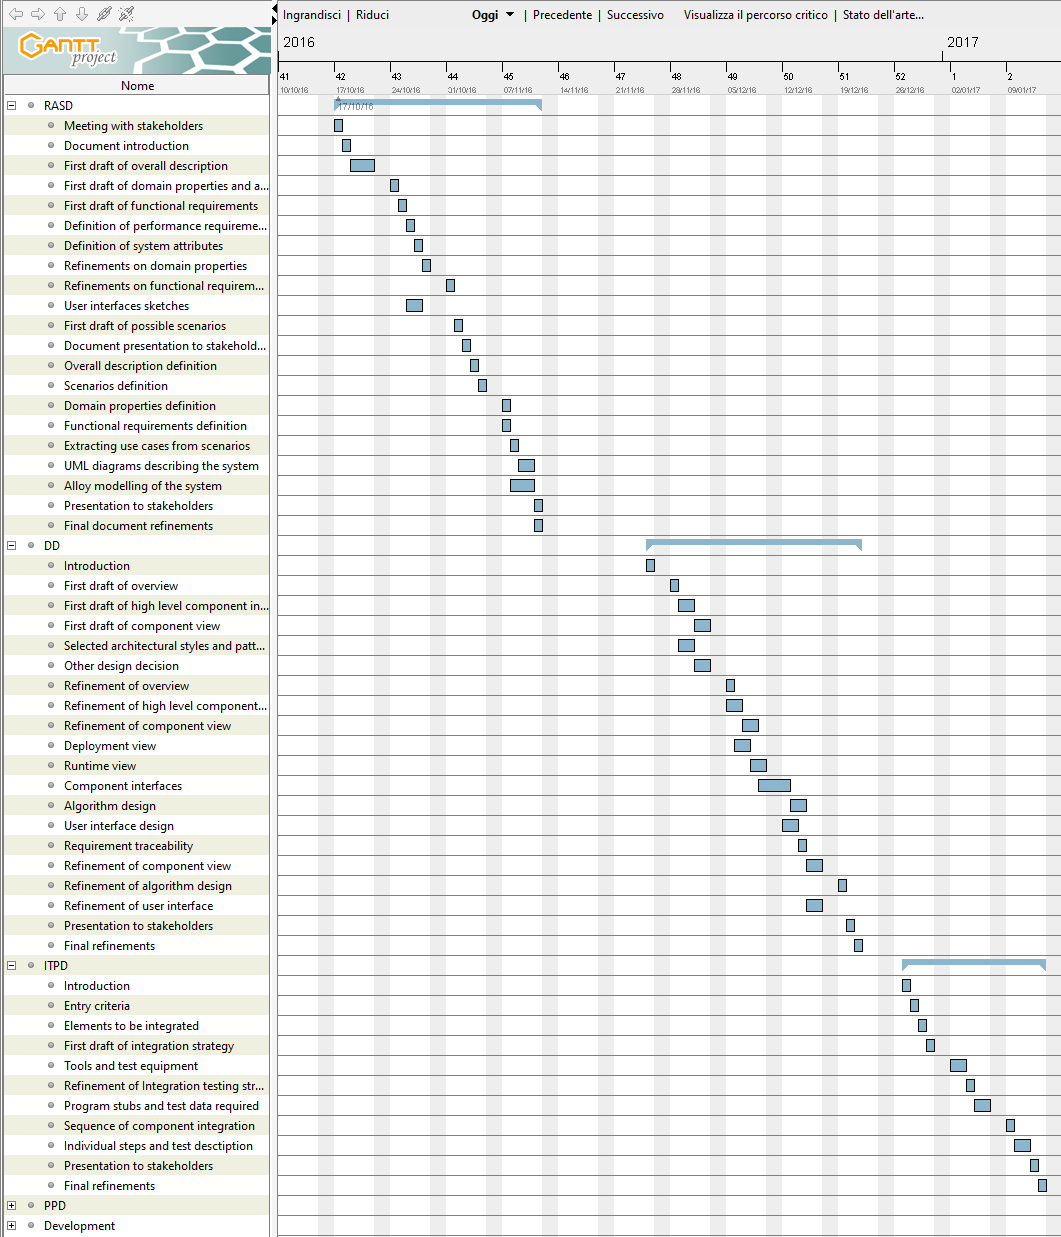
\includegraphics[width=500px]{../Datas/images/tasks-schedule-1.png}
	}
	\caption{Project tasks 1}
		\label{fig:tasks-1}
\end{figure}

\begin{figure}[H]
	\centerline{
		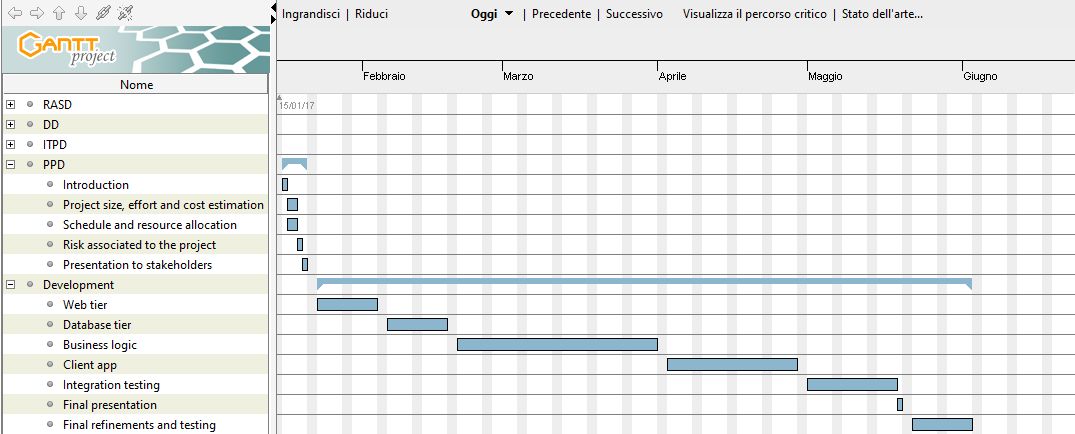
\includegraphics[width=500px]{../Datas/images/tasks-schedule-2.png}
	}
	\caption{Project tasks 2}
		\label{fig:tasks-2}
\end{figure}

\newpage
Following is a more accurate definition of each task deadline.

\begin{figure}[H]
	\centerline{
		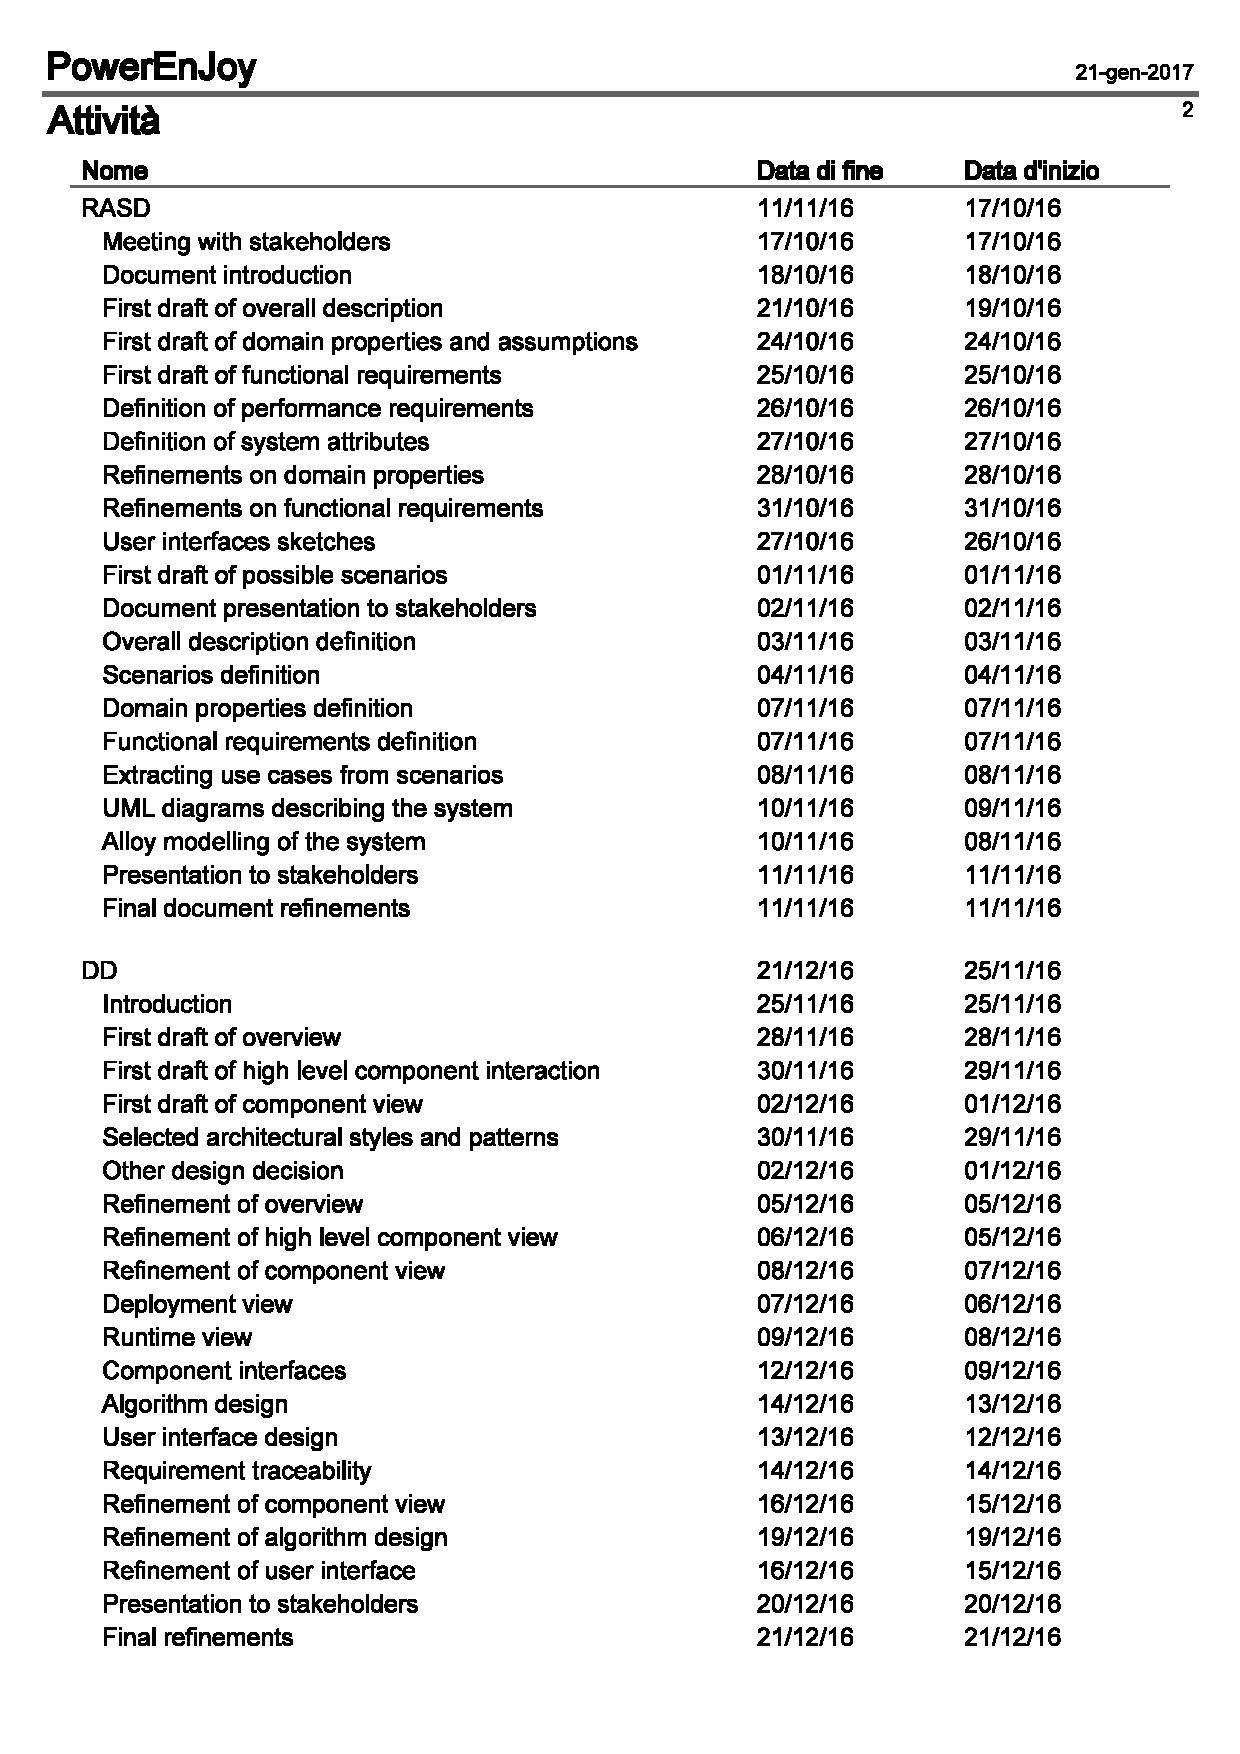
\includegraphics[width=371px]{../Datas/schedule-dates-1.pdf}
	}
		\label{fig:tasks-2}
\end{figure}

\begin{figure}[H]
	\centerline{
		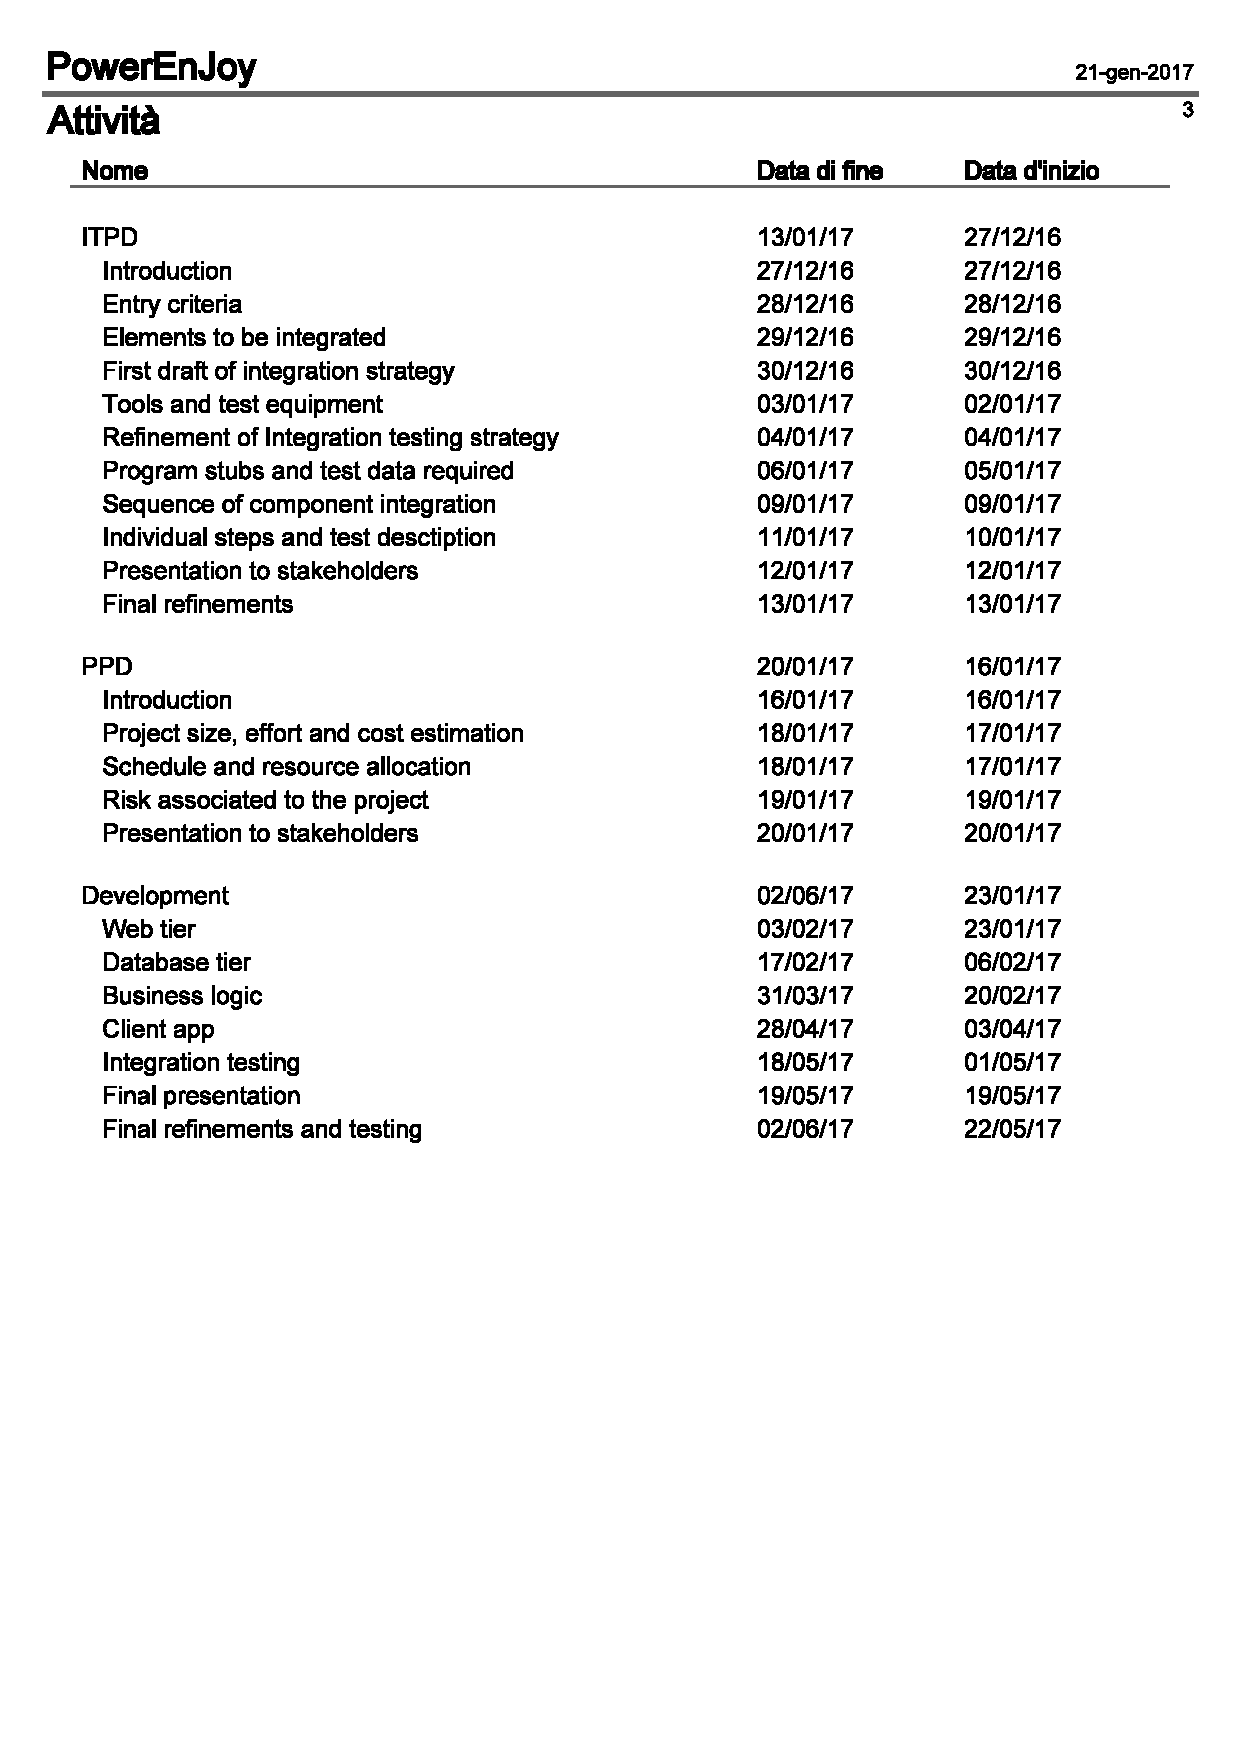
\includegraphics[width=400px]{../Datas/schedule-dates-2.pdf}
	}
		\label{fig:tasks-2}
\end{figure}
